\documentclass[UTF8,11pt,a4paper]{ctexart}

\usepackage[a4paper,top=2.05cm,bottom=2.15cm,left=2.15cm,right=2.15cm]{geometry}
\usepackage{amsmath,amssymb}
\usepackage{booktabs,tabularx,array,multirow}
\usepackage{graphicx,float,caption,subcaption}
\usepackage{tikz}
\usetikzlibrary{arrows.meta,positioning,fit}
\usepackage{xcolor}
\usepackage{enumitem}
\usepackage{fancyhdr}
\usepackage{hyperref}
\usepackage{siunitx}
\usepackage{microtype}

\definecolor{Ink}{HTML}{202532}
\definecolor{Muted}{HTML}{697386}
\definecolor{Blue}{HTML}{4F76C7}
\definecolor{Orange}{HTML}{CF6E3E}
\definecolor{Green}{HTML}{69AE34}
\definecolor{Rule}{HTML}{D9DEE8}
\definecolor{Panel}{HTML}{F5F7FA}

\hypersetup{
  colorlinks=true,
  linkcolor=Blue,
  urlcolor=Blue,
  citecolor=Blue,
  pdfauthor={},
  pdftitle={Lab5 GPU 编程实验报告}
}
\graphicspath{{figures/}}
\captionsetup{font=small,labelfont=bf,labelsep=quad}
\setlength{\parindent}{2em}
\setlength{\parskip}{0.18em}
\setlength{\emergencystretch}{2.5em}
\setlist{nosep,leftmargin=2.2em}
\renewcommand{\arraystretch}{1.18}
\sisetup{round-mode=places,round-precision=2,detect-all}

\pagestyle{fancy}
\fancyhf{}
\fancyhead[L]{并行程序设计 · Lab5 GPU 编程}
\fancyhead[R]{HIP 与 PCFG 端到端实验}
\fancyfoot[C]{\thepage}
\renewcommand{\headrulewidth}{0.4pt}
\setlength{\headheight}{14pt}

\newcommand{\code}[1]{\texttt{#1}}
\newcommand{\pass}{\textcolor{Green!70!black}{\textbf{PASS}}}
\newcommand{\meanstd}[2]{#1\,$\pm$\,#2}

\begin{document}

\begin{titlepage}
  \centering
  \vspace*{2.2cm}
  {\Large 并行程序设计课程实验报告\par}
  \vspace{1.4cm}
  {\fontsize{26}{34}\selectfont\bfseries Lab5：GPU 编程\par}
  \vspace{0.45cm}
  {\Large 基础 HIP 算法与真实 PCFG 口令生成加速\par}
  \vspace{1.4cm}
  \rule{0.82\textwidth}{0.7pt}
  \vspace{1.2cm}

  \begin{tabular}{>{\bfseries}p{3cm}p{8cm}}
    姓名： & 刘蔚霖 \\[0.3cm]
    学号： & 2412727 \\[0.3cm]
    实验平台： & AMD Radeon 8060S Graphics / ROCm HIP 7.13 \\[0.8cm]
    实验日期： & 2026 年 6 月 19 日 \\
  \end{tabular}

  \vfill
  {\color{Muted}x86-64 · 40 Compute Units · Wavefront Size 32\par}
\end{titlepage}

\begin{abstract}
本实验使用图形处理器（Graphics Processing Unit，GPU）和异构计算可移植接口（Heterogeneous-compute Interface for Portability，HIP），完成向量加法、矩阵转置、直方图、归约、Monte Carlo 积分与 K-Means 聚类六项基础实验，并构建概率上下文无关文法（Probabilistic Context-Free Grammar，PCFG）口令候选生成的 GPU 数据通路。PCFG 实验包含单概率模板（probabilistic template，PT）、多 PT 批处理、stream overlap、CPU/GPU 调度和真实模型端到端生成。六个 Notebook 均完整执行；四阶段合成实验的 80 条记录全部通过；真实 PCFG 实验以 RockYou 100 万行子集训练模型，解析 1,003,870 个口令，形成 9,888 个 PT，并在 199 个 WorkUnit 上取得 90/90 条正确记录。1M 候选规模下，4-PT batch 的墙钟时间为 \meanstd{42.92}{3.50} ms，同轮 CPU baseline 的中位加速比为 5.46×；默认调度的墙钟时间为 \meanstd{50.64}{7.38} ms，中位加速比为 4.77×。实验同时显示，小规模任务受传输和主机端结构转换支配，真实 overlap 路径还受到结果还原成本限制。本文基于分段计时、同轮配对加速比、哈希校验和路由守恒分析这些边界。

\noindent\textbf{关键词：} GPU；HIP；并行算法；PCFG；批处理；异构调度；性能分析
\end{abstract}

\setcounter{tocdepth}{1}
\tableofcontents
\clearpage

\section{技术摘要与主要结论}

本实验的核心问题是：数据并行 kernel 能否在正确生成结果的前提下，将 GPU 吞吐能力转化为端到端收益。基础实验覆盖连续访存、共享存储、原子操作、树形归约、随机采样和迭代聚类，用于验证线程组织、访存模式与同步策略。PCFG 实验进一步引入不规则任务大小、主机对象到连续缓冲区的转换、CPU/GPU 分流及输出顺序恢复，形成完整的异构执行链路。

实测结果支持四项主要结论。第一，GPU kernel 的局部优化能够直接改善设备端时间。向量加法在 128 threads/block 时取得最低平均 kernel 时间 0.0210 ms；归约从全局原子基线推进到每线程多元素方案后，时间由 0.0309 ms 降至 0.0124 ms。第二，访存位置决定高冲突算法的性能。10M/64 bins 和 100M/512 bins 两组直方图中，局部数据存储（Local Data Share，LDS）私有化方案分别比串行 CPU 快 12.83×和 12.82×，同时避免逐元素全局原子竞争。

第三，模块级 GPU 时间不能代替端到端时间。合成单 PT 实验中，1K 至 100K 候选的 H2D 传输保持在约 3.8--3.9 ms，固定成本掩盖了短 kernel 的并行收益。真实 1M 候选中，4-PT batch 的 GPU total 均值为 8.81 ms，而端到端墙钟时间为 42.92 ms；其差值来自 WorkUnit 转换、主机打包、输出还原和容器构造。第四，真实任务分布决定调度结果。默认阈值将 940,796 个候选分配到 GPU，将 59,204 个候选保留在 CPU；保守阈值高于全部 WorkUnit，因而形成纯 CPU 批处理路径。后者的比值反映 CPU 批处理相对逐项 baseline 的收益，不表示 GPU 加速。

\section{实验要求、平台、数据来源与计时口径}

\subsection{实验目标与验收方法}

实验目标分为三个层次。基础层验证六类典型 GPU 算法的正确性和性能特征；模块层验证 PCFG 单 PT、多 PT、overlap 和调度接口；系统层将真实训练模型、优先队列、WorkUnit 和 GPU 生成器连接为端到端流程。验收覆盖算法设计、平台说明、正确性、性能、瓶颈分析和适用边界。每项性能结论均对应保存的 Notebook 输出或结果文件。

正确性采用分层校验。基础 Notebook 检查数值误差、计数守恒或聚类迭代输出。合成 PCFG 使用 CPU 结果逐项比较，四阶段共 80 条 benchmark 记录均为 \pass。真实 PCFG 对候选数量、输出顺序和 Fowler--Noll--Vo（FNV）哈希进行校验；调度模式同时验证 GPU 候选数与 CPU 回退候选数之和等于目标数量。三个规模、六种模式、五次重复共 90 条记录全部为 \pass。

\subsection{硬件、软件与训练数据}

表~\ref{tab:platform} 汇总执行环境。计算单元（Compute Unit，CU）是 Radeon GPU 的基本执行资源；wavefront 表示按相同指令推进的一组工作项。本平台的 wavefront size 为 32，因此 block size 与 32 对齐有助于减少不足一个 wavefront 的线程浪费。

\begin{table}[H]
\centering
\caption{实验平台与软件环境}
\label{tab:platform}
\begin{tabularx}{0.92\textwidth}{>{\bfseries}p{3.5cm}X}
\toprule
项目 & 配置 \\
\midrule
主机架构 & x86-64 \\
GPU & AMD Radeon 8060S Graphics \\
执行资源 & 40 CU，wavefront size 32 \\
运行时与编译器 & ROCm/HIP 7.13，AMD clang 23.0.0git \\
基础实验 & 六个 Jupyter Notebook，完整保留代码、输出与图 \\
PCFG 训练输入 & RockYou 100 万行子集，文件大小 9,889,460 bytes \\
真实模型 & 解析口令 1,003,870；PT 9,888；WorkUnit 199 \\
重复次数 & 基础实验按 Notebook 设置；PCFG 每个配置 5 次 \\
\bottomrule
\end{tabularx}
\end{table}

PCFG 训练耗时 1,490.2235 ms，收集 1M 候选对应 WorkUnit 耗时 10.3692 ms。这两项为模型和任务准备成本，生成模式的墙钟时间从共享任务集准备完成后开始计量。六种模式复用完全相同的 WorkUnit 集合，避免优先队列状态变化影响比较。

\subsection{计时口径与统计量}

主机到设备（Host-to-Device，H2D）表示输入缓冲区传输；设备到主机（Device-to-Host，D2H）表示输出缓冲区传输。表~\ref{tab:timing} 给出各计时指标的边界。只有边界相同的指标参与 speedup 计算。

\begin{table}[H]
\centering
\caption{计时指标及其边界}
\label{tab:timing}
\begin{tabularx}{\textwidth}{>{\bfseries}p{3.1cm}p{5.5cm}X}
\toprule
指标 & 覆盖范围 & 用途 \\
\midrule
HIP event & 同一 HIP stream 内事件间隔 & H2D、kernel、D2H 分段计时 \\
GPU total & H2D + kernel + D2H & 比较设备通路的模块级成本 \\
主机处理 & WorkUnit 转换、连续化、结果还原 & 解释 prepare、pack 与 unpack 成本 \\
End-to-end wall time & 单个生成模式函数的完整墙钟时间 & 真实 PCFG 六模式同轮比较 \\
Shell wall time & 进程启动、脚本和输入输出在内的墙钟时间 & Monte Carlo、K-Means 的独立负载说明 \\
Paired speedup & 同一重复轮次 CPU wall / 模式 wall & 控制 CPU baseline 的轮次波动 \\
\bottomrule
\end{tabularx}
\end{table}

PCFG 表格同时报告均值、样本标准差和中位数。均值与标准差描述运行波动；中位配对 speedup 作为主要比较指标。1M CPU baseline 的首轮冷启动单独分析，repeats 2--5 用于稳态敏感性检查。

\section{六项 HIP 基础实验}

\subsection{Vector Add：线程组织与有效带宽}

向量加法 kernel 以全局线程索引定位元素，并执行 $C_i=A_i+B_i$。每个元素读取两个单精度输入并写回一个单精度输出，因此有效带宽按式~\eqref{eq:bw} 计算，其中 $N=1{,}048{,}576$，$t$ 为 kernel 时间。
\begin{equation}
  B_{\mathrm{eff}}=\frac{12N}{t}\,.
  \label{eq:bw}
\end{equation}

图~\ref{fig:vector} 展示 block size 对 kernel 时间和有效带宽的影响，误差线为 10 次测量的一个标准差。
\begin{figure}[H]
  \centering
  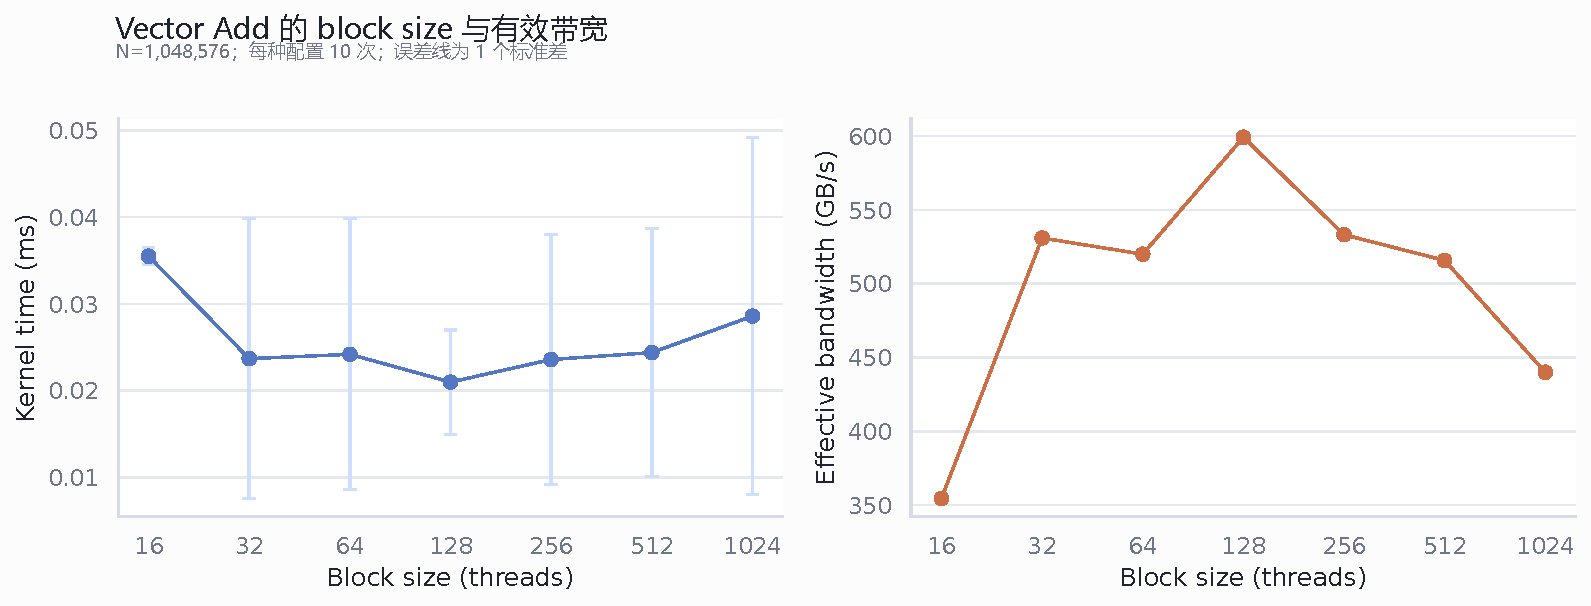
\includegraphics[width=\textwidth]{basic_vector_add.pdf}
  \caption{Vector Add 的 block size、kernel 时间与有效带宽}
  \label{fig:vector}
\end{figure}

128 threads/block 的平均时间最低，为 0.0210 ms，对应约 599 GB/s 的按算法字节量计算的有效带宽。32 至 512 threads/block 的均值处于 0.0210--0.0244 ms，说明连续访存使多个 block 配置均能保持较高吞吐。16 和 1024 threads/block 分别受到 wavefront 利用率与每 block 资源占用影响，时间均值较高。有效带宽是基于读写字节量和 HIP event 时间的派生指标，用于同一 kernel 内部比较。

\subsection{Matrix Transpose：连续访问与规模效应}

矩阵转置 kernel 使用二维线程索引 $(idx,idy)$，从 \code{input[idy*cols+idx]} 连续读取，并写入 \code{output[idx*rows+idy]}。同一行线程的输入访问连续，输出访问以 rows 为跨度。图~\ref{fig:transpose} 报告该直接转置 kernel 的总时间和单位元素成本，从而区分矩阵规模与单元素效率。
\begin{figure}[H]
  \centering
  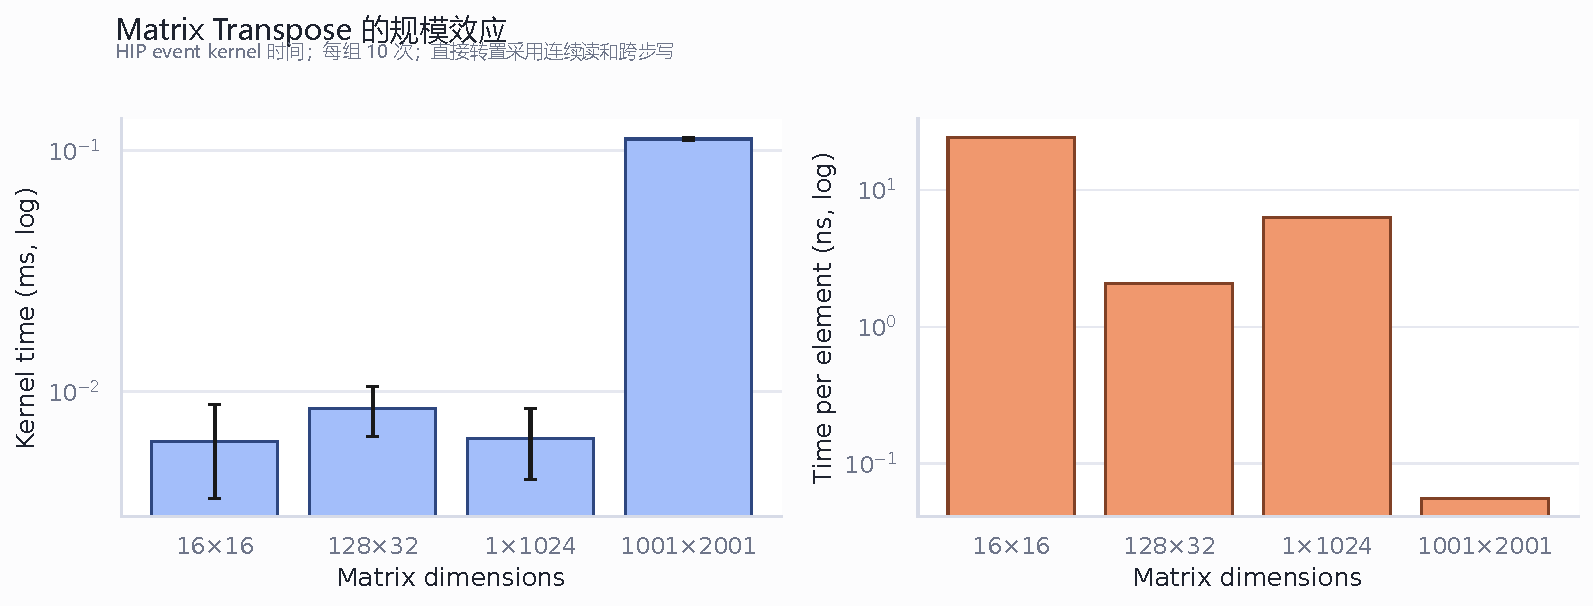
\includegraphics[width=\textwidth]{basic_transpose.pdf}
  \caption{Matrix Transpose 的总时间与单位元素成本}
  \label{fig:transpose}
\end{figure}

16×16、128×32、1×1024 和 1001×2001 的平均 kernel 时间依次为 0.0062、0.0085、0.0064 和 0.1119 ms。1001×2001 矩阵的总时间最高，但其单位元素成本最低，说明较大工作量提高了并行资源利用率并摊薄 launch 成本。1×1024 的长条形输入仍保持 0.0064 ms，表明边界判断能够处理非方阵和退化维度。

\subsection{Histogram：全局原子与 LDS 私有化}

直方图比较串行 CPU、逐元素全局原子和 LDS 私有化三种实现。LDS 是 CU 内工作组共享的低延迟存储。优化 kernel 先在每个工作组建立私有直方图，再将局部结果合并到全局 bins，从而把高频原子冲突从全局存储转移到片上存储。图~\ref{fig:histogram} 给出两种规模的时间与相对串行 CPU 的 speedup。
\begin{figure}[H]
  \centering
  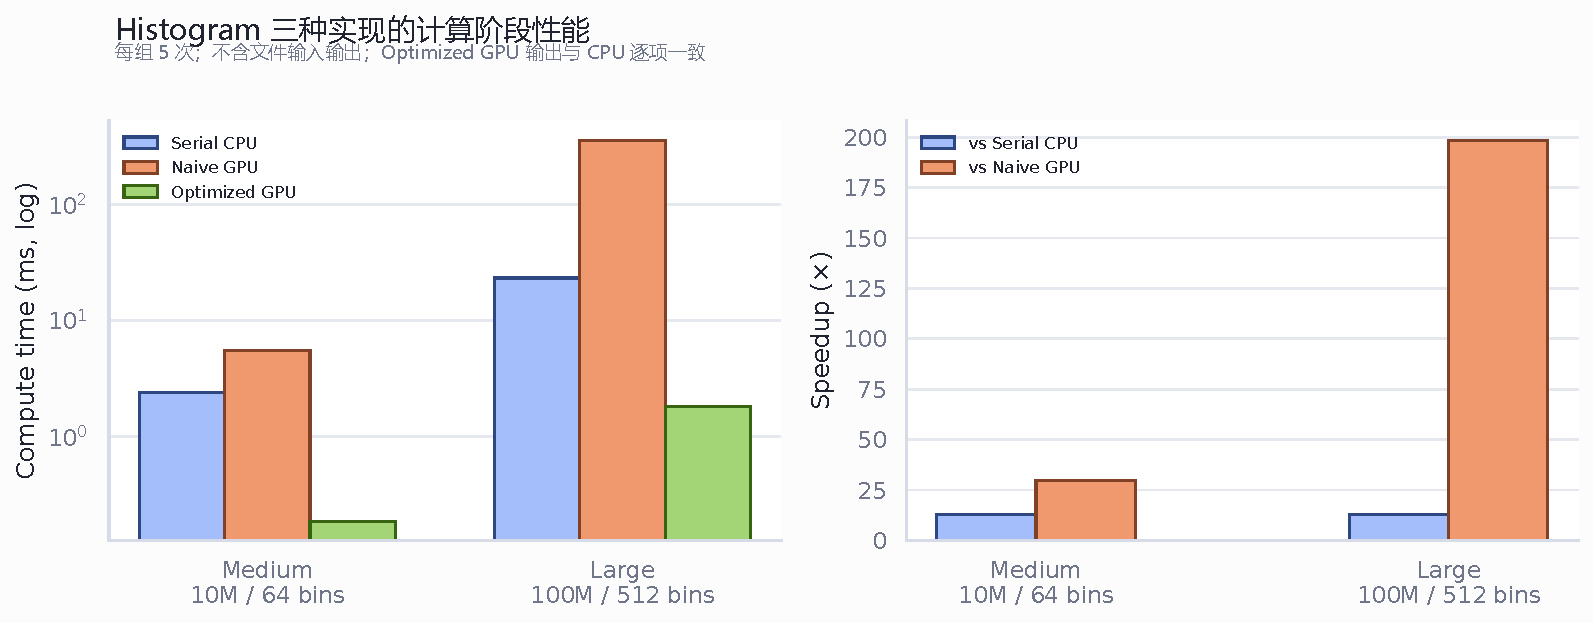
\includegraphics[width=\textwidth]{basic_histogram.pdf}
  \caption{Histogram 三种实现的时间与 speedup}
  \label{fig:histogram}
\end{figure}

10M 输入、64 bins 时，串行 CPU、全局原子和 LDS 私有化时间分别为 2.3936、5.5709 和 0.1866 ms；对应标准差为 0.0872、0.0113 和 0.0014 ms。100M 输入、512 bins 时三者分别为 23.3382、360.7488 和 1.8208 ms；对应标准差为 0.3905、0.6555 和 0.0463 ms。LDS 方案在两组规模上分别取得 12.83×和 12.82×；全局原子方案在大规模下比 LDS 方案慢 198.13×。该结果直接反映原子冲突位置对吞吐的影响。

\subsection{Reduction：同步范围与 wavefront shuffle}

归约将 1M 个输入压缩为单个和。四种策略依次为全局原子基线、LDS 树形归约、加入 wavefront shuffle 的树形归约和每线程多元素处理。图~\ref{fig:reduction} 展示策略推进过程中的 kernel 时间和相对首个方案的 speedup。
\begin{figure}[H]
  \centering
  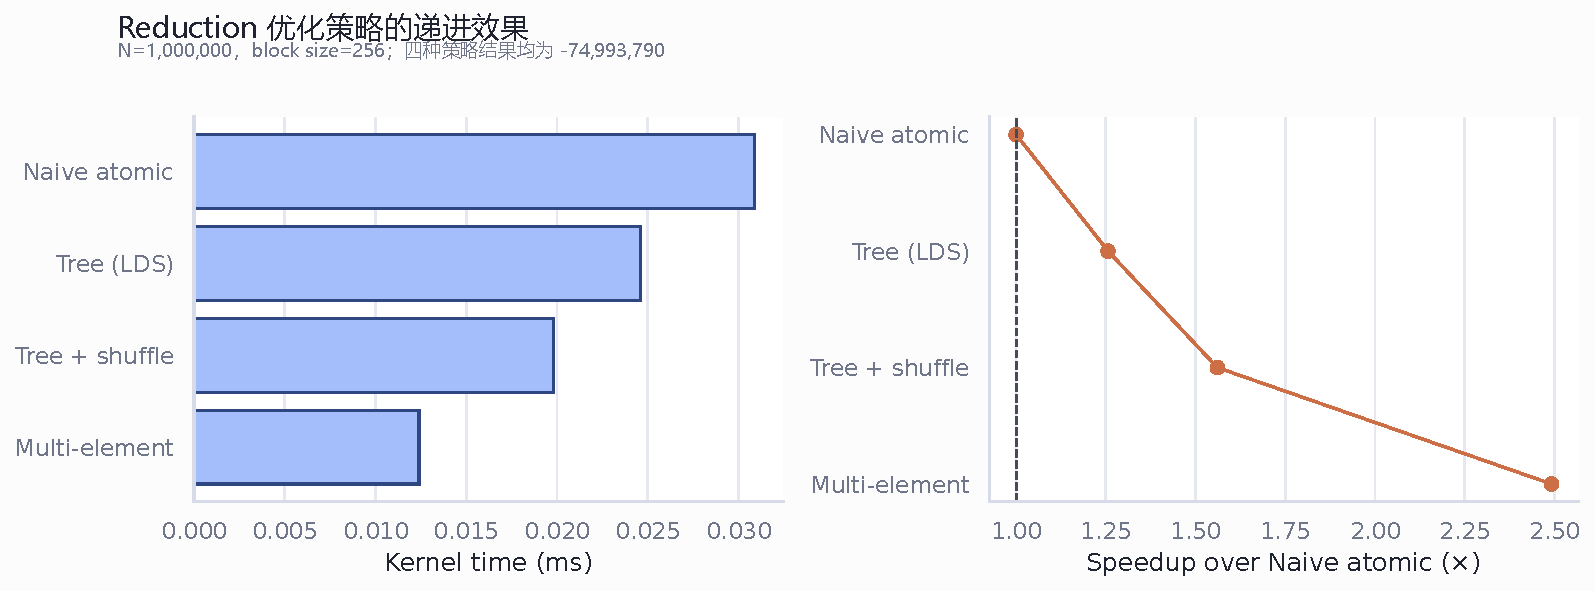
\includegraphics[width=\textwidth]{basic_reduction.pdf}
  \caption{Reduction 四种策略的性能递进}
  \label{fig:reduction}
\end{figure}

四种方案的平均时间依次为 0.0309、0.0246、0.0198 和 0.0124 ms，对应 1.00×、1.26×、1.56×和 2.49×。wavefront shuffle 允许寄存器值在线程间交换，使树形归约由 0.0246 ms 降至 0.0198 ms；每线程多元素处理进一步减少参与归约的中间值。四种实现的结果均为 $-74{,}993{,}790$，验证了性能变化没有改变归约值。

\subsection{Monte Carlo 与 K-Means：规模和工作负载}

Monte Carlo 通过并行采样估计积分，K-Means 通过并行距离计算和簇统计更新中心。图~\ref{fig:scaling} 左侧给出 Monte Carlo 的 shell wall time，右侧给出 K-Means 在 $N=50{,}000$、$k=50$ 时的工作量。本组 K-Means 只有一个带时间记录的规模，因此右图用于说明负载组成，不推断规模趋势。
\begin{figure}[H]
  \centering
  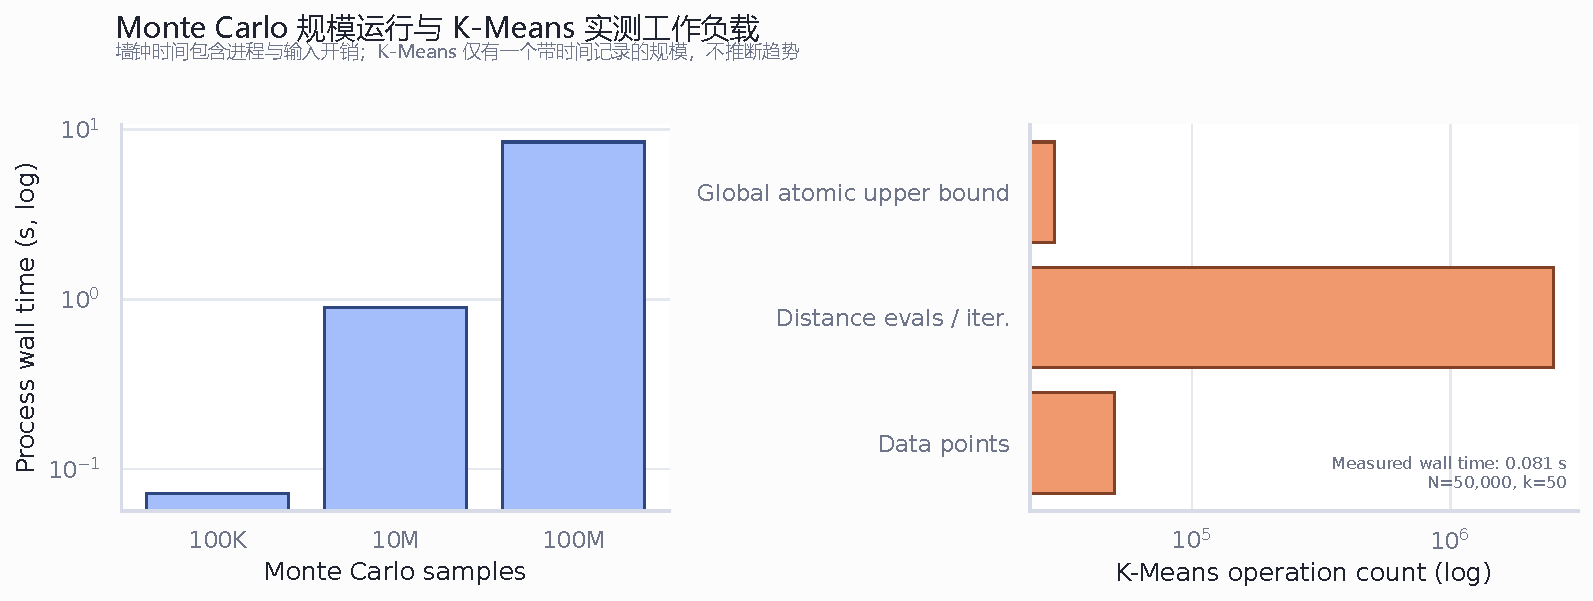
\includegraphics[width=\textwidth]{basic_scaling.pdf}
  \caption{Monte Carlo 规模运行与 K-Means 实测工作负载}
  \label{fig:scaling}
\end{figure}

Monte Carlo 在 100K、10M 和 100M 样本下的墙钟时间分别为 0.072、0.894 和 8.454 s。10M 到 100M 的样本数与时间均约增长 10 倍，表明大规模区间主要由采样计算支配。K-Means 单次迭代包含 250 万次点--中心距离计算；196 个 block 对簇统计执行的全局原子操作上界为 29,400 次，测得墙钟时间为 0.081 s。该配置展示了规则距离计算与不规则簇更新同时存在的负载结构。

\section{PCFG 数据结构、kernel 与 CPU/GPU 数据流}

\subsection{真实任务到 GPU 批次的映射}

PCFG 模型将口令表示为字母、数字和符号片段的组合，并按概率维护 PT。\code{PriorityQueue} 保存按概率排序的 PT；\code{WorkUnit} 由一个 PT 和半开区间 $[begin,end)$ 构成，用于限定末段候选值范围。CPU baseline 调用 \code{GenerateRange} 生成该区间内的全部候选。

GPU 适配层将 WorkUnit 转换为 \code{PcfgGpuPtBatch}。该结构包含已由前置片段构成的 \code{prefix}，以及末段区间对应的 \code{values}。主机打包器将字符串对象转换为固定槽宽的连续缓冲区：prefix 最大 64 bytes，value 最大 32 bytes，输出最大 65 bytes（含终止符）。长度超限的 PT 进入 CPU 回退路径，并计入回退数量。

\subsection{kernel 索引与批处理布局}

多 PT kernel 为每个候选分配一个工作项。主机端保存每个 PT 的候选偏移，工作项由全局索引查找所属 PT，随后读取对应 prefix 和 value，将二者写入固定槽宽输出缓冲区。该设计使候选值和输出槽位保持连续，线程之间没有写冲突。单 PT 接口复用同一批处理 kernel；多 PT 接口通过一次 launch 合并多个短任务。

图~\ref{fig:dataflow} 展示从模型训练到结果验证的端到端数据流，并标出 CPU 与 GPU 的职责边界。
\begin{figure}[H]
\centering
\begin{tikzpicture}[
  node distance=8mm and 8mm,
  box/.style={draw=Rule,very thick,rounded corners=2pt,fill=Panel,minimum height=9mm,align=center,font=\small,inner xsep=6pt},
  cpu/.style={box,draw=Orange!75,fill=Orange!8},
  gpu/.style={box,draw=Blue!75,fill=Blue!8},
  arrow/.style={-{Stealth[length=2.2mm]},thick,draw=Muted}
]
\node[cpu] (train) {RockYou 训练\\PCFG model};
\node[cpu,right=of train] (queue) {PriorityQueue\\PT 排序};
\node[cpu,right=of queue] (units) {WorkUnit\\$[begin,end)$};
\node[cpu,right=of units] (prepare) {prefix + values\\合法性与调度};
\node[gpu,below=12mm of prepare] (pack) {连续缓冲区\\host pack};
\node[gpu,left=of pack] (h2d) {H2D};
\node[gpu,left=of h2d] (kernel) {HIP kernel\\prefix + value};
\node[gpu,left=of kernel] (d2h) {D2H};
\node[cpu,below=12mm of d2h] (unpack) {host unpack\\恢复 string};
\node[cpu,right=of unpack] (merge) {CPU 回退合并\\顺序恢复};
\node[cpu,right=of merge] (verify) {数量 + FNV\\正确性验证};

\draw[arrow] (train)--(queue);
\draw[arrow] (queue)--(units);
\draw[arrow] (units)--(prepare);
\draw[arrow] (prepare)--(pack);
\draw[arrow] (pack)--(h2d);
\draw[arrow] (h2d)--(kernel);
\draw[arrow] (kernel)--(d2h);
\draw[arrow] (d2h)--(unpack);
\draw[arrow] (unpack)--(merge);
\draw[arrow] (merge)--(verify);
\end{tikzpicture}
\caption{真实 PCFG 候选生成的 CPU/GPU 数据流}
\label{fig:dataflow}
\end{figure}

图中的 GPU total 仅覆盖 H2D、kernel 和 D2H。小任务或长度超限任务从合法性检查阶段进入 CPU 回退；端到端墙钟时间还包含 WorkUnit 转换、调度、host pack、host unpack、CPU 回退和输出合并。该边界解释了设备端时间较短时，端到端收益仍可能受主机对象处理限制。

\subsection{批处理、overlap 与调度策略}

多 PT 批处理将若干 \code{PcfgGpuPtBatch} 合并为一次传输和 launch。overlap 接口使用异步复制与 HIP stream 处理多个 chunk，使下一批打包或 CPU 工作与设备通路重叠。默认调度参数为 $min=4{,}096$、$target=65{,}536$、$max=131{,}072$：小于 min 的任务进入 CPU，累计值接近 target 时形成 GPU chunk，大于 max 的任务分片。保守参数为 $131{,}072/262{,}144/524{,}288$，用于观察更高 GPU 门槛下的路由结果。

\section{四阶段模块级实验}

\subsection{Stage 1：单 PT 与传输分解}

Stage 1 使用合成 prefix 和候选值，验证单 PT 的 CPU/GPU 一致性，并将 GPU total 分解为 H2D、kernel 和 D2H。图~\ref{fig:stage1} 展示 1K、10K 和 100K 候选的五次均值。
\begin{figure}[H]
  \centering
  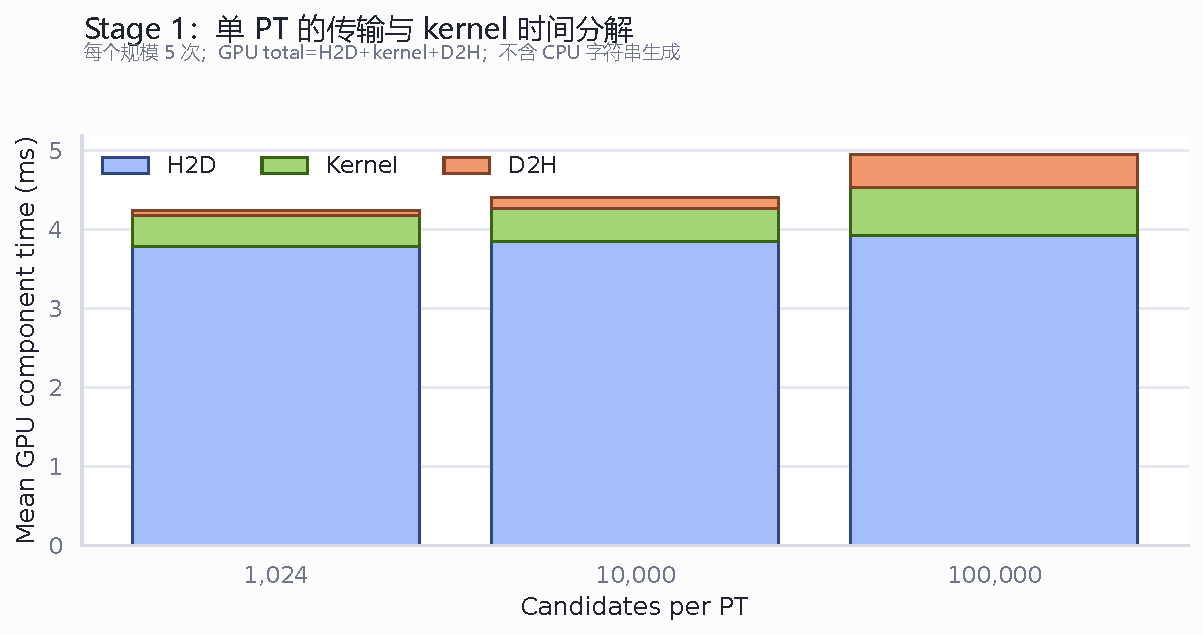
\includegraphics[width=\textwidth]{pcfg_stage1_breakdown.pdf}
  \caption{Stage 1 单 PT 的 H2D、kernel 与 D2H 分解}
  \label{fig:stage1}
\end{figure}

表~\ref{tab:stage1} 给出精确统计。H2D 从 1K 的 3.7828 ms 到 100K 的 3.9194 ms，仅增加 0.1366 ms；其在 GPU total 中的占比仍为 79.3\%。100K 的 CPU/GPU 比值为 0.3084，说明该模块在本规模内尚未摊薄设备分配与传输固定成本。

\begin{table}[H]
\centering
\caption{Stage 1 单 PT 五次运行均值}
\label{tab:stage1}
\begin{tabular}{rrrrrrr}
\toprule
候选数 & CPU/ms & H2D/ms & kernel/ms & D2H/ms & GPU total/ms & CPU/GPU \\
\midrule
1,024   & 0.0107 & 3.7828 & 0.3973 & 0.0584 & 4.2385 & 0.0026 \\
10,000  & 0.1365 & 3.8475 & 0.4127 & 0.1491 & 4.4093 & 0.0310 \\
100,000 & 1.5182 & 3.9194 & 0.6108 & 0.4150 & 4.9452 & 0.3084 \\
\bottomrule
\end{tabular}
\end{table}

\subsection{Stage 2--3：多 PT 合并与 stream overlap}

Stage 2 在相同候选总数下比较单 PT 与多 PT 合并；Stage 3 比较顺序多 PT 和 stream overlap。每个 PT 含 10K 个 value，PT 数为 2、4 和 8。图~\ref{fig:stage23} 把两个问题并列展示。
\begin{figure}[H]
  \centering
  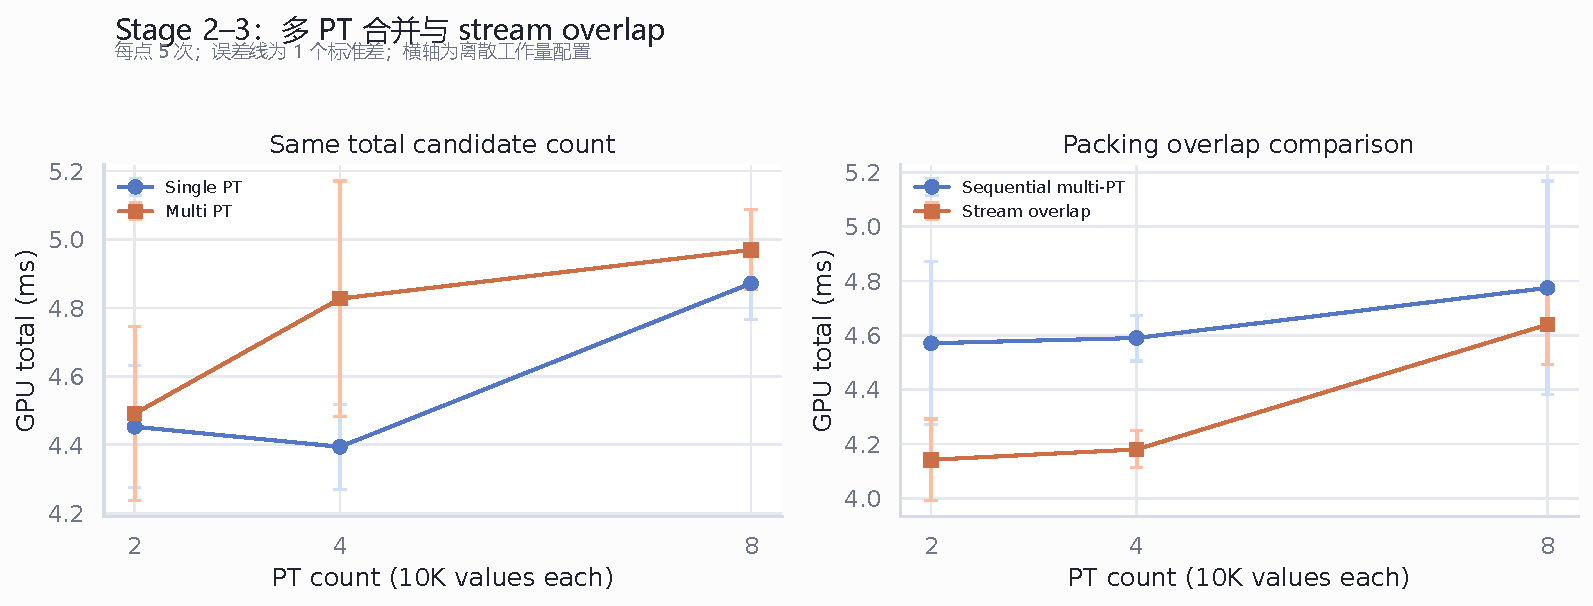
\includegraphics[width=\textwidth]{pcfg_stage23_compare.pdf}
  \caption{Stage 2--3 的同工作量批处理与 overlap 比较}
  \label{fig:stage23}
\end{figure}

Stage 2 中，多 PT GPU total 均值为 4.4909、4.8270 和 4.9696 ms；同总候选数的单 PT 均值为 4.4528、4.3941 和 4.8716 ms。多 PT 元数据和偏移数组引入额外传输，短任务合并尚未产生稳定收益。Stage 3 中，顺序多 PT 的均值为 4.5709、4.5902 和 4.7747 ms，overlap 均值为 4.1425、4.1805 和 4.6396 ms，分别缩短 9.4\%、8.9\%和 2.8\%。这组数据只覆盖设备通路；真实字符串还原成本在端到端实验中单独计量。

\subsection{Stage 4：调度与数量守恒}

Stage 4 使用大小不均的合成 PT 验证调度器。每轮共有 67,264 个候选，其中 1,168 个进入 CPU，66,096 个进入 GPU；五次运行的候选数量和输出内容全部一致。CPU 全量生成时间为 \meanstd{1.6401}{0.0437} ms，调度路径墙钟时间为 \meanstd{34.2969}{2.7434} ms，CPU/GPU 比值为 \meanstd{0.0480}{0.0036}。GPU total 仅为 \meanstd{4.8490}{0.2549} ms，而完整调度时间明显更高，说明小对象分组、输出容器构造与顺序恢复是该合成配置的主要成本。

四阶段共获得 80 条 benchmark 记录：Stage 1 为 15 条，Stage 2 为 30 条，Stage 3 为 30 条，Stage 4 为 5 条。所有记录均为 \pass，且没有 HIP error 或编译错误。模块级数据说明固定开销和主机数据布局是进入真实端到端实验前必须量化的因素。

\section{真实 PCFG 端到端实验}

\subsection{训练模型、共享任务集与 WorkUnit 分布}

真实实验从 RockYou 100 万行子集训练 PCFG 模型，解析 1,003,870 个口令，得到 9,888 个 PT。优先队列按概率收集同一批 WorkUnit，并分别截取 10K、100K 和 1M 候选规模。训练耗时 1,490.2235 ms，收集 1M 候选任务耗时 10.3692 ms；二者在所有模式间共享。

图~\ref{fig:ptdist} 展示三个候选规模的 WorkUnit 候选数分位点，并叠加默认和保守调度的 min 阈值。
\begin{figure}[H]
  \centering
  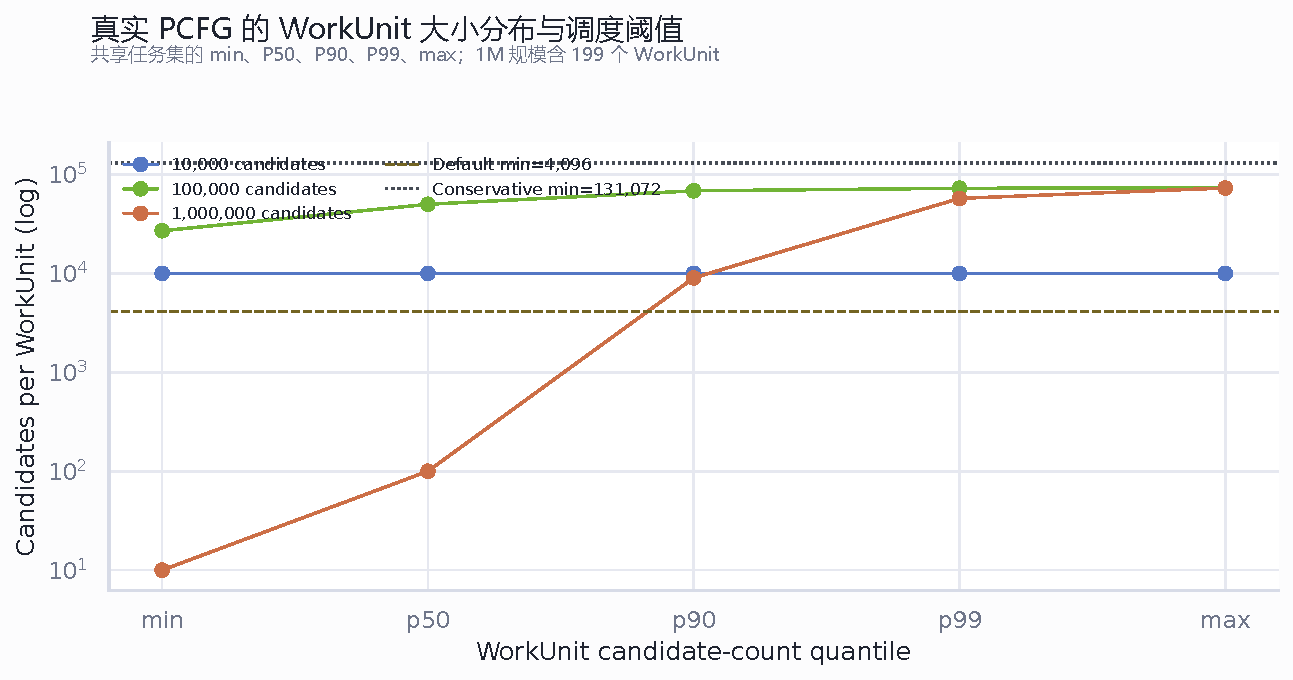
\includegraphics[width=\textwidth]{pcfg_real_pt_distribution.pdf}
  \caption{真实 WorkUnit 大小分布与调度阈值}
  \label{fig:ptdist}
\end{figure}

10K 规模只有一个 10,000 候选的 WorkUnit。100K 规模包含两个 WorkUnit，候选数为 26,998 和 73,002。1M 规模包含 199 个 WorkUnit，min、P50、P90、P99 和 max 分别为 10、100、9,004、57,364.38 和 73,002。默认 min=4,096 将中大型 WorkUnit 送入 GPU，并将长尾中的小任务留在 CPU。保守 min=131,072 高于最大 WorkUnit，因此所有任务进入 CPU 路径。

\subsection{六种模式的墙钟时间与配对 speedup}

六种模式为 CPU \code{GenerateRange} baseline、单 PT GPU、4-PT batch、4-PT overlap、默认调度和保守调度。每种模式在每个规模运行五次。图~\ref{fig:realperf} 左侧报告端到端墙钟时间均值及标准差，右侧报告相对同轮 CPU baseline 的中位 speedup 和四分位区间。
\begin{figure}[H]
  \centering
  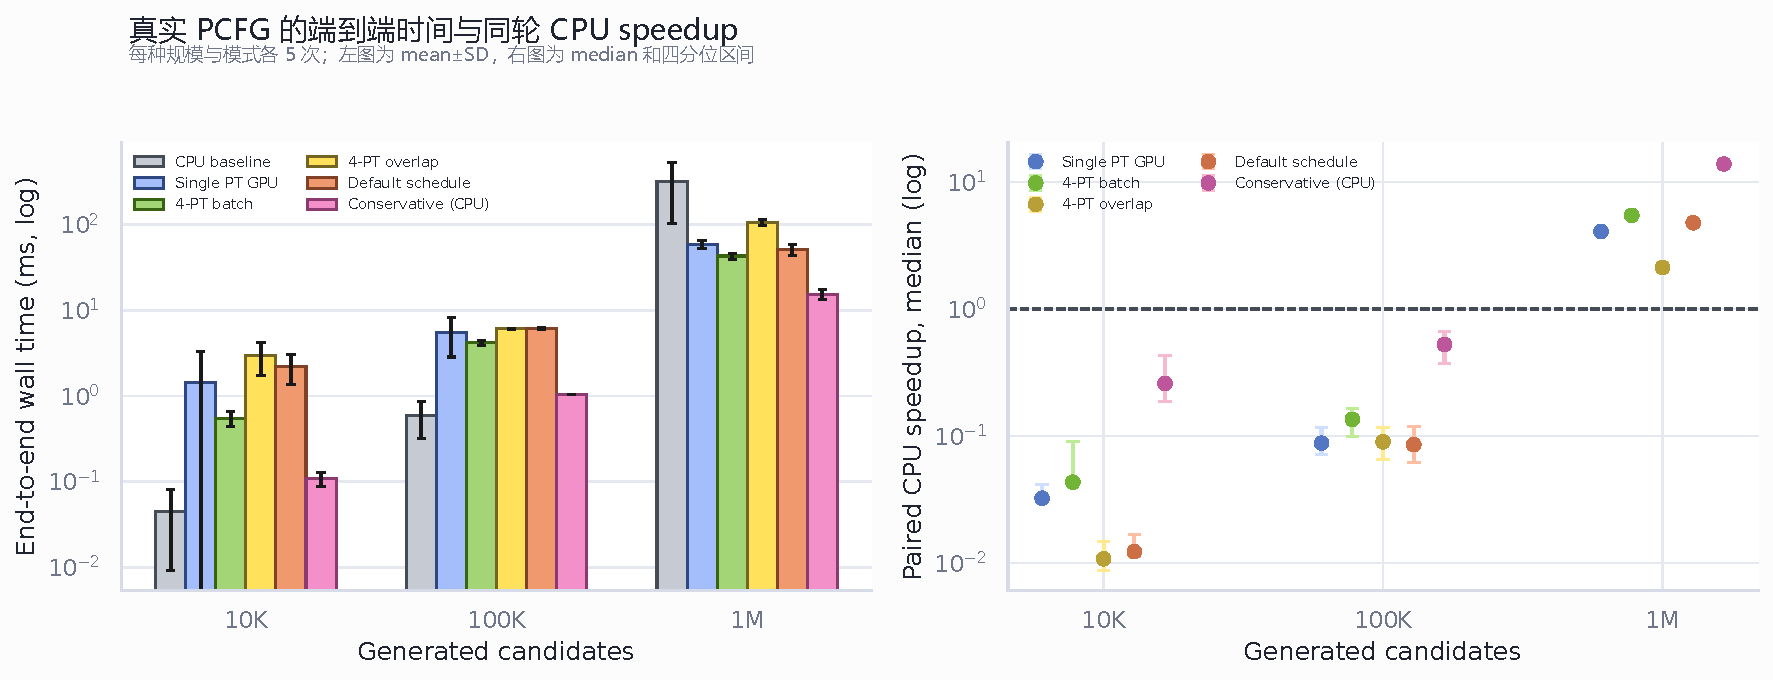
\includegraphics[width=\textwidth]{pcfg_real_performance.pdf}
  \caption{真实 PCFG 六种模式的墙钟时间与同轮 CPU speedup}
  \label{fig:realperf}
\end{figure}

10K 和 100K 规模下，GPU 模式的 speedup 均小于 1，表明转换、launch 和输出恢复成本超过并行收益。1M 规模跨过收益边界：4-PT batch 的平均墙钟时间最低于 GPU 模式，为 \meanstd{42.92}{3.50} ms，中位 speedup 为 5.46×；单 PT GPU 为 \meanstd{58.84}{5.87} ms 和 4.07×；默认调度为 \meanstd{50.64}{7.38} ms 和 4.77×。4-PT overlap 的墙钟时间为 \meanstd{105.56}{7.78} ms，中位 speedup 为 2.13×，仍快于 CPU baseline，但慢于顺序 4-PT batch。

表~\ref{tab:real1m} 给出 1M 规模的精确统计和分流数据。保守调度的 15.31 ms 来自纯 CPU 批处理路径；其 13.84×中位比值衡量批处理相对逐 WorkUnit \code{GenerateRange} baseline 的差异。

\begin{table}[H]
\centering
\caption{真实 PCFG 1M 候选五次运行结果}
\label{tab:real1m}
\small
\begin{tabular}{lrrrrr}
\toprule
模式 & Wall mean±SD/ms & Median speedup & GPU 候选 & CPU 候选 & PASS \\
\midrule
CPU baseline       & $313.56\pm209.95$ & 1.00  & 0       & 1,000,000 & 5/5 \\
Single PT GPU      & $58.84\pm5.87$    & 4.07  & 1,000,000 & 0       & 5/5 \\
4-PT batch         & $42.92\pm3.50$    & 5.46  & 1,000,000 & 0       & 5/5 \\
4-PT overlap       & $105.56\pm7.78$   & 2.13  & 1,000,000 & 0       & 5/5 \\
Default schedule   & $50.64\pm7.38$    & 4.77  & 940,796 & 59,204  & 5/5 \\
Conservative (CPU) & $15.31\pm2.01$    & 13.84 & 0       & 1,000,000 & 5/5 \\
\bottomrule
\end{tabular}
\end{table}

\subsection{CPU/GPU 分流与端到端开销解释}

图~\ref{fig:routing} 将 1M 候选的 CPU/GPU 分流归一化为比例。该图区分 GPU 批处理收益和 CPU 批处理收益，避免把路由策略的结果归因于单一设备。
\begin{figure}[H]
  \centering
  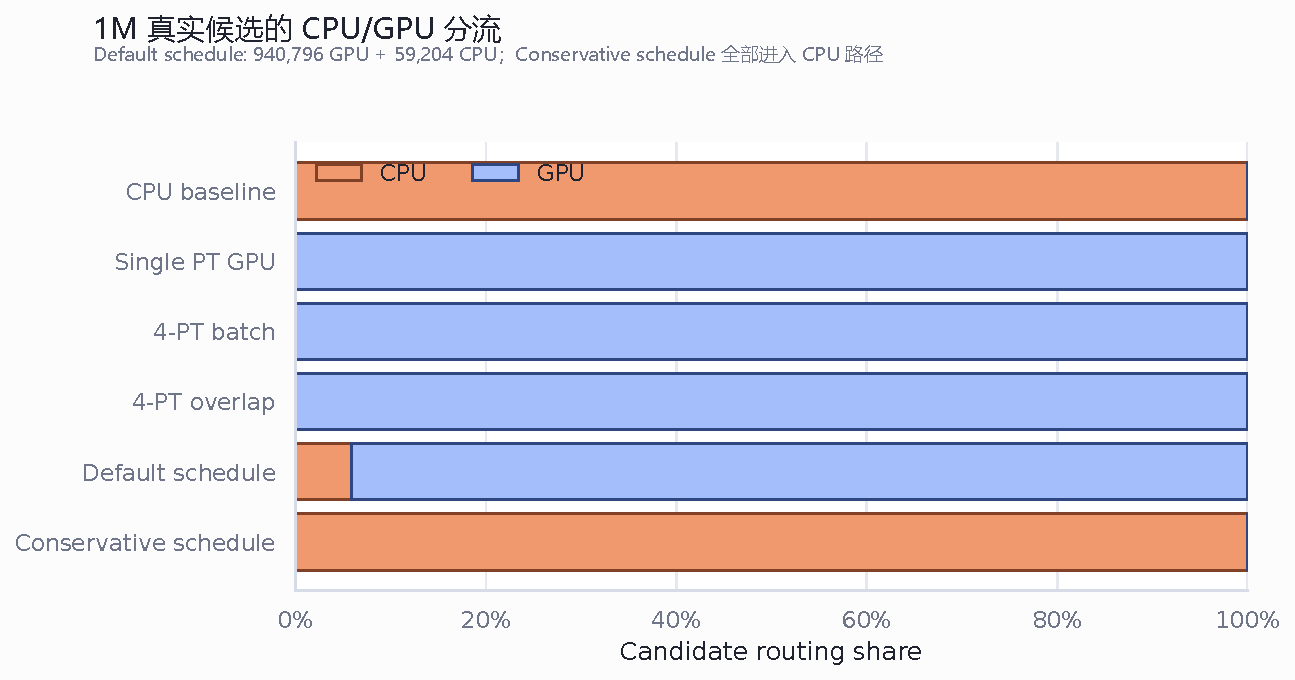
\includegraphics[width=\textwidth]{pcfg_real_routing.pdf}
  \caption{1M 真实候选在各模式中的 CPU/GPU 分流}
  \label{fig:routing}
\end{figure}

Single PT、4-PT batch 和 4-PT overlap 将全部候选送入 GPU。默认调度使用 48 个 GPU WorkUnit 和 151 个 CPU WorkUnit；前者虽然数量较少，却承载 94.08\% 的候选，说明阈值按候选数而非 WorkUnit 数量分流能够把大任务集中到 GPU。保守调度的 199 个 WorkUnit 全部进入 CPU，显示阈值与真实任务分布必须配套选择。

4-PT batch 在 1M 规模下的 H2D、kernel、D2H 均值分别为 3.97、1.49 和 3.34 ms，GPU total 为 8.81 ms。4-PT overlap 的 GPU total 为 9.80 ms，host unpack 均值达到 62.52 ms，因此异步 stream 没有转化为更低端到端时间。默认调度的 GPU total 为 5.45 ms，host unpack 为 21.92 ms，并另有 CPU 回退工作。当前数据结构中，输出先写入固定槽宽缓冲区，再逐项构造 \code{std::string}；这一还原过程是 1M overlap 路径的主要墙钟成本。

\subsection{冷启动与稳态敏感性}

1M CPU baseline 的五次运行存在明显首轮效应。图~\ref{fig:cold} 展示各重复轮次，并以虚线标出 repeats 2--5 的均值。
\begin{figure}[H]
  \centering
  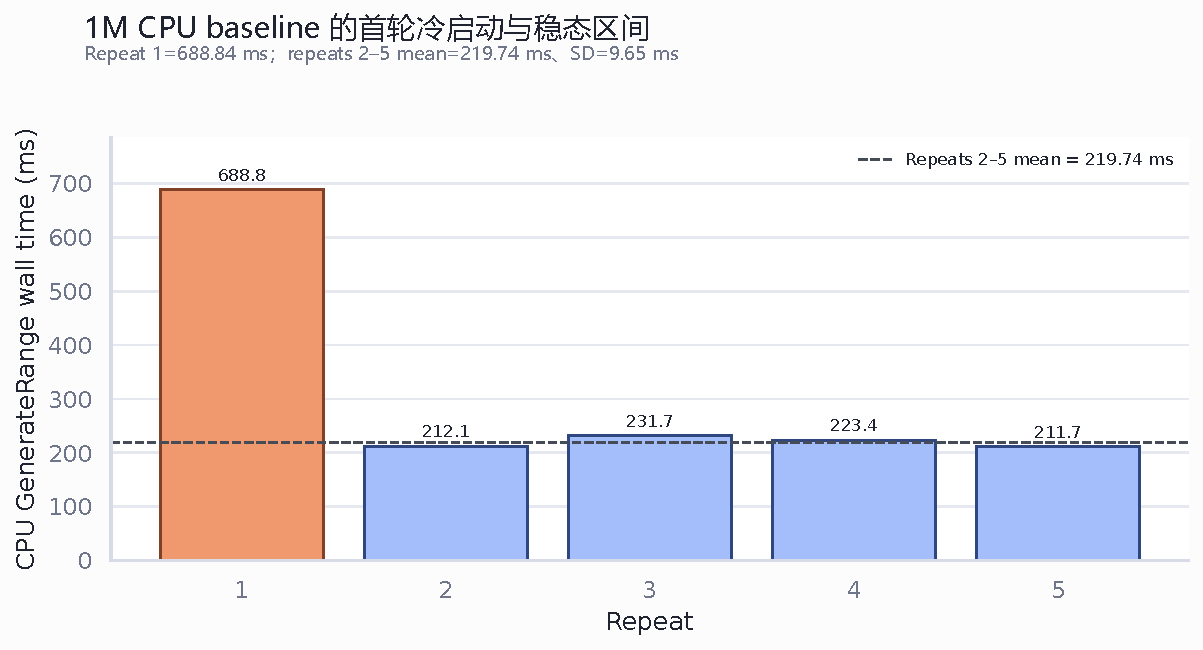
\includegraphics[width=\textwidth]{pcfg_real_cold_start.pdf}
  \caption{1M CPU baseline 的首轮冷启动与稳态区间}
  \label{fig:cold}
\end{figure}

首轮为 688.84 ms，repeats 2--5 的均值为 \meanstd{219.74}{9.65} ms，中位数为 217.75 ms。首轮约为稳态均值的 3.14 倍，可能包含分配器、页映射和缓存状态建立成本。使用 repeats 2--5 重新计算同轮中位 speedup 后，Single PT、4-PT batch、4-PT overlap 和默认调度分别为 4.02×、5.37×、2.10×和 4.66×；相对排序保持一致。保守 CPU 批处理路径为 13.58×，其设备归属仍为 CPU。

\subsection{正确性与复现性检查}

真实记录覆盖 $3\times6\times5=90$ 个配置点。每条记录均满足候选总数一致、FNV 哈希一致和 CPU/GPU 分流数量守恒；运行汇总为 \code{status=PASS}、\code{benchmark\_rows=90}、\code{failures=0}。调度模式在合并后按任务标识恢复顺序，再与 CPU baseline 比较。独立的合成回归测试同时保持通过，说明真实数据接入没有改变单 PT、多 PT、overlap 和调度接口的基本语义。

\section{局限性、适用边界与结论}

\subsection{实验边界}

本实验的性能结论适用于 Radeon 8060S、HIP 7.13 和当前固定槽宽数据布局。基础 Notebook 的 HIP event 时间用于 kernel 内部比较；Monte Carlo 与 K-Means 的 shell wall time包含进程与输入输出成本，两者不与 HIP event 时间计算 speedup。K-Means 只有一个带时间记录的规模，报告据此描述单规模工作量。

PCFG 的训练和任务收集是一次性准备成本，生成阶段的 wall time不包含这两项。对于只生成少量候选的一次性调用，1.49 s 的训练成本占主导；对于复用模型的连续生成服务，生成阶段数据更能代表稳定运行成本。合成 PT 四阶段用于隔离 GPU 模块行为，真实 PT 实验用于评价对象转换、调度、回退和结果还原共同组成的端到端路径。

固定槽宽布局简化了 kernel 索引并保证连续写入，同时为短字符串保留未使用空间。prefix 超过 64 bytes、value 超过 32 bytes或拼接结果超过 64 bytes 的任务进入 CPU 回退。真实 1M 任务中未出现破坏数量守恒的超长输入；其他训练集的字符串长度分布可能改变 GPU 可处理比例。MPI 与 ARM NEON MD5 属于口令猜测系统的其他执行边界，不参与 Radeon 8060S 的时间比较。

\subsection{结论}

六项基础实验验证了 GPU 性能由线程组织、访存连续性、片上共享存储、同步范围和任务规模共同决定。Vector Add 和 Reduction 展示 block 配置与 wavefront 操作的影响；Histogram 展示 LDS 私有化对高冲突原子操作的决定性作用；Matrix Transpose、Monte Carlo 和 K-Means 展示规模、形状与工作负载组成对利用率的影响。

PCFG 端到端实验表明，GPU 候选拼接 kernel 能够在 1M 规模产生可验证收益，4-PT batch 取得 5.46×同轮中位 speedup。10K 与 100K 规模仍由传输和主机对象处理主导。默认调度根据 WorkUnit 候选数把 94.08\% 的候选分配到 GPU，并保持数量、顺序和 FNV 哈希一致。overlap 的设备并发收益受到 host unpack 限制；保守调度的较短时间来自纯 CPU 批处理。由此，当前系统的有效策略是：复用训练模型，以候选数阈值合并足够大的 WorkUnit，优先采用多 PT 批处理，并以端到端墙钟时间和同轮 CPU baseline 评价收益。

\end{document}
